Im Folgenden werden die Resultate der durchgeführten Simulationen analysiert. Ziel ist es, eine Erklärung für den Übergang zwischen den vorgestellten Wachstumsregionen des kapillaren Aufstiegs zu finden. Insbesondere wird der Übergang vom linearen Bereich ($z(t)\sim t$) zum von Lucas und Washburn beschriebenen Wachstum ($z(t)\sim \sqrt{t}$) betrachtet. Um potenzielle Einflüsse durch verschiedene Kontaktwinkel zu berücksichtigen, wurden die Simulationen mit drei unterschiedlichen Werten durchgeführt. Zusätzlich wurden Simulationen mit aktivierten Ungleichgewichtsrandbedingungen durchgeführt, um den Einfluss einer Relaxation an der Wand auf den kapillaren Aufstieg zu analysieren. Zunächst wird die Gleichgewichtsrandbedingung in Kapitel \ref{sec: EquilibriumBoundaryCondition} untersucht, gefolgt von einem Vergleich mit der Ungleichgewichtsrandbedingung im Abschnitt \ref{sec: outOfEquilibriumBoundaryCondition}.

\section{Vorarbeiten}
Um einflüsse oder mögliche Fehlerquellen für die Simulationen zu identifizieren, wurden zunächst einige Vorarbeiten durchgeführt.
Die wichtigste und aufwendigste Vorarbeit ist es parameter zu finden, für die die Ergebnisse zum einen Pysikalisch, die simulationszeit aber nicht darunter leidet. Dazu wurde zunächst versucht den Kapillaren aufstieg mit dem Lucas Washburn Verhalten zu vergleichen. Da hier bereits schnell klar wurde, dass dies aus mehreren, genannten Gründen nciht funktionieren wird, erfolgten simulationen in denen die Mobilität und das Rechennetz variiert wurden. Außerdem wurde auch die verwenedung eines Adaptiven Netzes geprüft


Bei den verwendeten Dimensionen der Kapillare und der Flüssigkeiten, ist zu erwarten, dass der Einfluss der Gravitation vernachlässigbar ist, was auch in gesondert durchgeführten Simulationen gezeigt werden konnte, jedoch aufgrund der geringen aussagekraft eines Vergleichs mit Simulationen ohne Gravitation nicht weiter betrachtet wird. Damit wird jedoch auch klar, dass eine der besprochenen von Lucas und Washburn angenommen Vereinfachnungen für diesen Fall nicht gilt und eine Abweichung der vorhersage gemäß Gleichung \ref{eq: LW-Eq} darauf zurückzuführen ist, dass ein Gleichgewicht zwischen Kapillarkraft und viskosem drag nicht ausreicht, um den Kapillaren Aufstieg in frühen imbibitionsstadien zu beschreiben.

\section{Equilibrium Boundary Condition} 
\label{sec: EquilibriumBoundaryCondition}
Die auswertung mit nur einem der verwendeten Kontatkwinkel findet im folgenden mit einem Gleichgewichtskontaktwinkel von $\theta_{\mathrm{e}}=15^{\circ}$ statt. Ein Vergleich der Simulationsergebnisse für diesen Kontaktwinkel mit der Lucas-Washburn-Gleichung \ref{eq: LW-Eq} ist in Abbildung \ref{fig: LW-PFF_comp} dargestellt. Die vorhergesagte imbibition länge wird in rot und die Ergebnisse der Simulation in schwarz abgebildet. Um die gleiche Größenordnung wie die Simulation vorherzusagen, musste ein Korrekturfaktor zur Lucas-Washburn-Gleichung hinzugefügt werden.
\todo{Bild anpassen}
\begin{figure}[h]
    \centering
    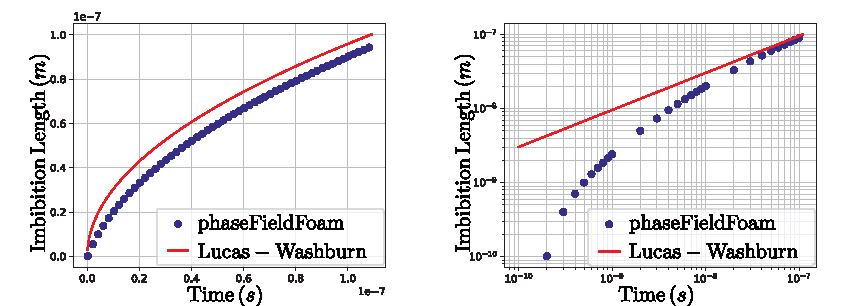
\includegraphics[width=.95\textwidth]{Pictures/LW-lin_loglog.pdf}
    \caption{Vergleich des von Lucas-Washburn vorhergesagten Wachstums mit den Ergenissen von \texttt{phaseFieldFoam}}
    \label{fig: LW-PFF_comp}
\end{figure}
In Abbildung \ref{fig: LW-PFF_comp} (a) erfolgt eine lineare und in \ref{fig: LW-PFF_comp} (b) eine logarithmische Skalierung. In der logarithmischen Darstellung werden die Unterschiede noch deutlicher. Anfangs ist die Steigung der Simulationsergebnisse größer als die der Vorhersage, bis sie schließlich konvergieren. Dies deutet darauf hin, dass der kapillare Aufstieg erst nach einer gewissen Zeit dem bekannten Lucas-Washburn-Wachstum folgt, was auch von vielen in Abschnitt \ref{sec: capillaryRise} zitierten Arbeiten bestätigt wird. 

Um die Unterschiede im Verhalten zu verstehen, ist es sinnvoll, die in der Wassersäule wirkenden Kräfte zu betrachten. Delanoy et al. \cite{delannoy2019DualRoleViscosity} führten diese Unterschiede auf eine lokale Dissipation zurück. Daher ist es ratsam, den Bereich nahe der Schnittstelle genauer zu betrachten. In Abbildung \ref{fig: eDiss_wedge} werden die viskosen Kräfte in der Wassersäule nahe der Kontaktlinie dargestellt. Dieser Bereich wird fokussiert, da in anderen Teilen der Wassersäule die Kräfte deutlich geringer sind. Es ist deutlich zu erkennen, dass nahe der Kontaktlinie und direkt an der Wand die viskosen Kräfte am größten sind. Es bilden sich zwei dissipative Kanäle aus. Hier überlagern sich die viskosen Kräfte nahe der Kontaktlinie und der viskosie Widerstand, hervorgerufen durch die Veränderungen des Kontaktwinkels aufgrund der Dynamik des Systems. \todo{check!!!!}

\begin{figure}[h]
    \centering
    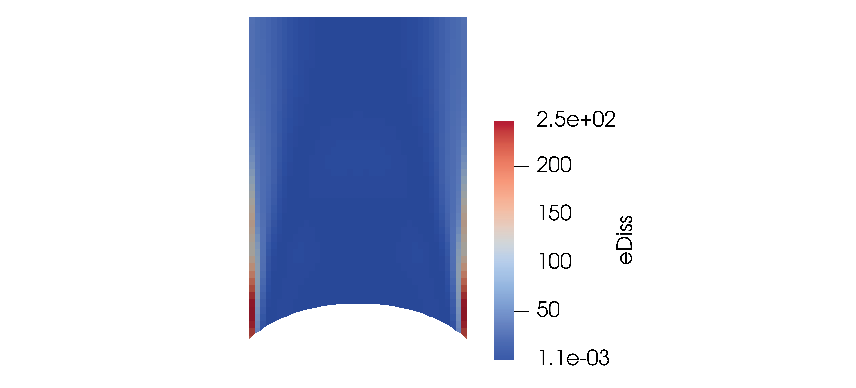
\includegraphics[width=.95\textwidth]{Pictures/eDiss_Wedge.pdf}
    \caption{Dissipative channels near the contact line.}
    \label{fig: eDiss_wedge}
\end{figure}

\begin{figure}[h]
    \centering
    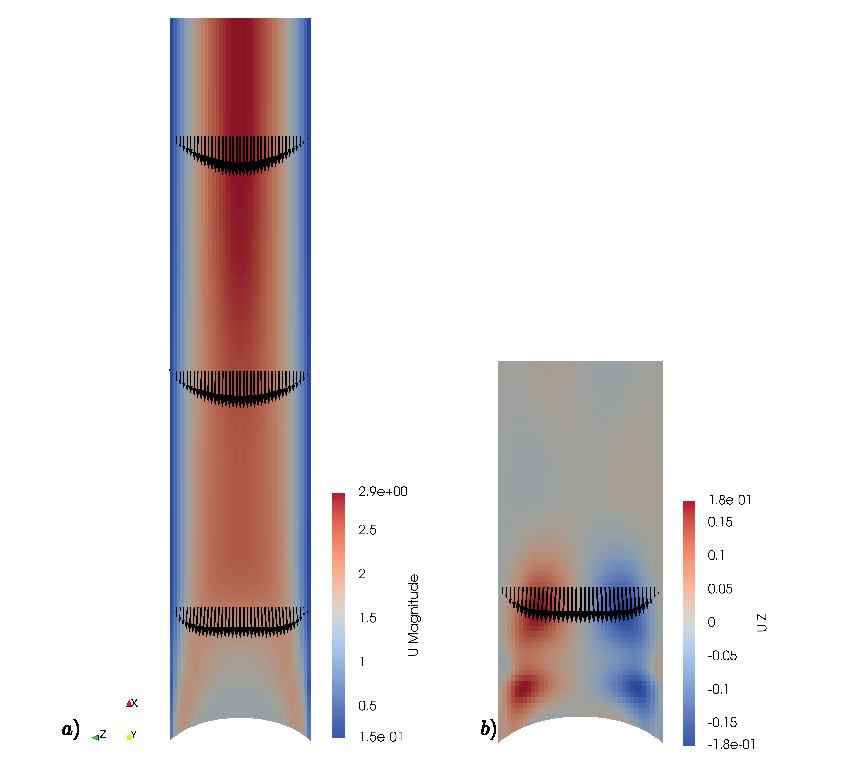
\includegraphics[width=.95\textwidth]{Pictures/Velo_Wedge.pdf}
    \caption{(a) Velocity field in the water column at $100ns$ and $\theta_{\mathrm{e}}=15^{\circ}$, (b) detailed view of recirculation near the interface.}
    \label{fig: Velofield_Wedge}
\end{figure}
In Abbildung \ref{fig: Velofield_Wedge} wird das Geschwindigkeitsfeld im Wasser visualisiert und entspricht den Erwartungen. In der Mitte der Kapillare ist die Geschwindigkeit des Wassers am höchsten (vgl. (a)). Zur Visualisierung des sich verändernden Geschwindigkeitsfeldes bei annäherung an das Interface wurden ebenfalls für drei Ebenen die Vektoren des Geschwindigkeitsfeldes hinzugefügt. Weit vom Interface entfernt, liegt das erwartete parabolische Profil vor. Bei näherung an das Interface ist deutlich zu erkennen wie die Strömung in der Mitte abgebremst wird und bei genauer betrachtung ist anhand der Vektoren auch zu erkennen, dass die Strömung an den Rand abgelenkt wird. Dazu wurde in (b) der Ausschnitt nahe des Interface vergrößert und statt der Magnitude der Geschwindigkeit nur die Komponente normal zur Strömungsrichtung ($z$-Richtung) visualisiert. Es ist deutlich zu erkennen, dass bis kurz vor der Strömung diese Komponente vernachlässigbar ist und nahe des Interface stark ansteigt und zwei Regionen zu bilden scheint. Eine direkt am Interface und nahe der Wand und ein weiteres etwas weiter innerhalb der Wassersäule. Anahnd der Legende ist deutlich erkennbar, dass die Größenordnung im Vergleich zur Geschwindigkeit in Strömungsrichtung sich um eine Dekade unterscheidet. Der Bereich in dem die Änderung der Geschwindigkeit stattfindet, wir im folgenden als $\mathrm{W}$ bezeichent. Bis zu diesem Bereich kann angenommen werden, dass die Strömung der von poiseuille beschriebenen entspricht und damit der Viskose Widerstand dem Poseuille viskosen Widerstand entspricht. Damit können dann die in $\mathrm{W}$ herrschenden viskosen Kräfte direkt aus der Simulation berechnet werden. Die insgesamt wirkenden viskosen Kräfte erhält man aus der Simulation mit Gleichung \ref*{eq: total_viscForce} und den viskosen Wiederstand kann man mit $F_{\eta}$ aus Gleichung \ref*{eq: NewtonBalanceForcesOnly} berechnen. Die Differenz der beiden Kräfte entspricht dann den in $\mathrm{W}$ herrschenden viskosen Kräften. 
Darüber hinaus wird mittels der Geschwindigkeit des Meniskus auch der theoretische, Poiseuille viskose Widerstand und die Widerstandkräfte am Meniskus (Gleichung \todo{EQ}) berechnet. Hierbei wird die von Cox und Voinov beschriebene Gleichung (\ref*{eq: Cox-Voinov}) zur Vorhersage des dynamischen Kontaktwinkels verwendet. Das Verhältnis der Längenskalen ist meist schwer abzuschätzen, da für $l_{\mathrm{m}}$ meist eine Länge von $1nm$ angenommen wird und für $l$ mehrere Lägen, wie der Radius, die Länge der Kapillare oder auch die Länge von $\mathrm{W}$ wird im folgenden ein Verhältnis von $l_{\mathrm{m}}/l\approx10$ angenommen. 
\todo{Woher kommt das?}
\todo{Bild oder beschrieben der rezikulation} 

\begin{figure}[h]
    \centering
    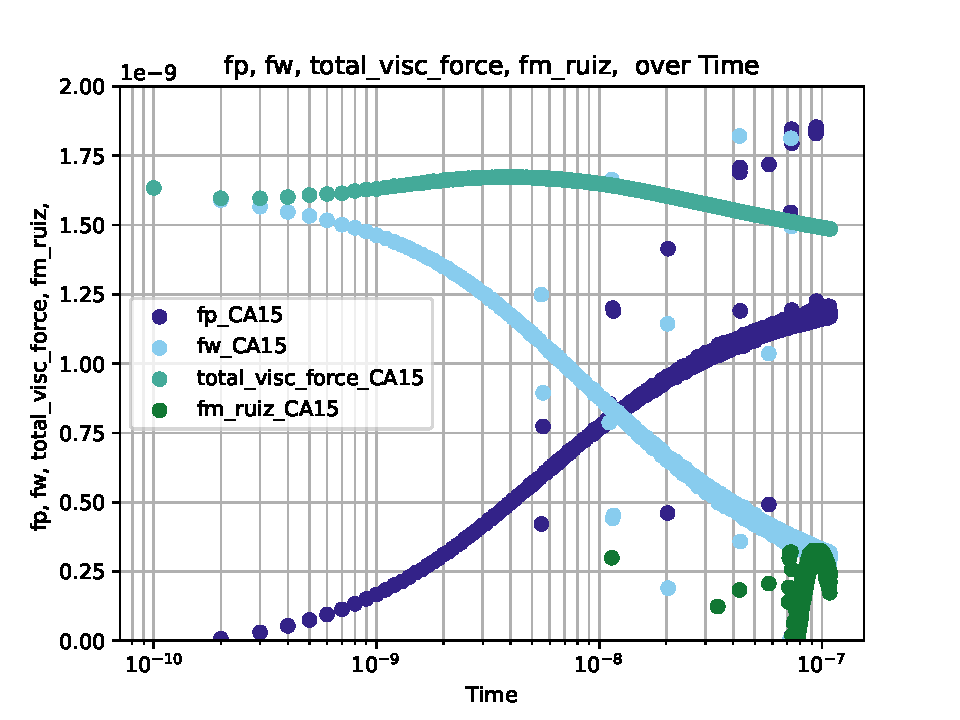
\includegraphics[width=.95\textwidth]{Pictures/log_fp_fw_total_visc_force_fm_ruiz_overTime.pdf}
    \caption{Viscous forces over time}
    \label{fig: forcesOverTime}
\end{figure}




Plottet man diese Kräfte in einem Diagramm wird deutlich, wie zu Beginn der imbibition die Kräfte aus der Meniskusbildung die viskosen Kräfte überwiegen und erst nach einiger Zeit die viskosen Kräfte dominant werden. Dazu wurden in Abbildung \ref*{fig: forcesOverTime} auch die Ergebnisse aus der theoretischen Berechnung anhand der Simulationsdaten und der direkt aus der Simulation stammenden Daten gezeigt. Delanoy hat postuliert, dass ab einer imbibitionslänge von $\sim r\cdot ln(r/l_s)$ die viskosen Kräfte überwiegen. Auf diesen Fall übertragen würde das bedeuteten, dass für $t\approx 3\cdot 10^{-9}$ die viskosen Kräfte überwiegen. Dies entspricht nicht den Ergebnissen der Simulation, ist aber durchaus plausibel, da zum einen Ruiz-Gutiérrez et al. \cite{ruiz2019CapillaryRise} eine postuliert hat, dass dieser Bereich durchaus früher beginnen kann und die Annahme einer korrekte charaktertischen Weglänge schwierig ist und in vielen Bereichen in denen eine solche Größe verwendet wird zu Problemen führt. \todo{check and talk with Francisco about this; especially about how he computed ruiz fm thing. Mine is shit i assume...}



Zur Berechnung des Kontaktwinkels kann die in Kapitel \ref*{chap: Validation} vorgestellte Methode zur Berechnung des Radius der spähre verwendet werden. Wie in Kapitel \ref*{chap: wettingTheory} beschrieben wird davon ausgegangen, dass sich der Meniskus zu einem Kreissegment entwickelt. Da in diesem Fall nur der Kontaktwinkel benötigt wird, kann auf eine in \cite{buttPhysicsChemistryInterfaces} vorgestellte Gleichung zurückgegriffen werden, womit sich der Kontaktwinkel mit 
\begin{equation}
    \theta = 90^{\circ}- 2\tan^{-1}\left(\frac{h}{R}\right) 
\end{equation}
berechnen lässt. Die variablen und wie sie erhalten werden ist bereits in Kapitel \ref*{chap: Validation} beschrieben. \todo{add cox angles to compare in one plot and just 15deg case}
\begin{figure}[h]
    \centering
    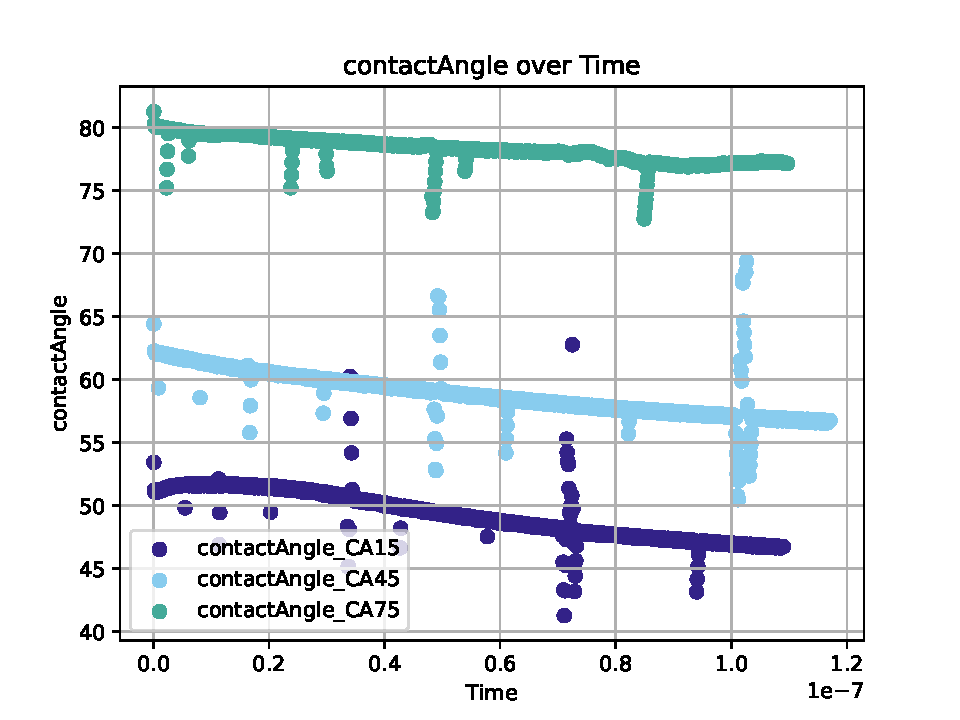
\includegraphics[width=.95\textwidth]{Pictures/contactAngle_overTime.pdf}
    \caption{computed contact angle over time }
    \label{fig: CA_overTime}
\end{figure}
Darin ist zu sehen, dass sich sehr schnell ein Winkel einstellt,... \todo{ausformulieren mit Daten vom feineren Netz.}


%Diese erkenntnis bestätigt sich, wenn man die Steigung der SImulaiton an einigen Stichproben ermittelt. Dabei wird deutlich, dass die Steigung asymptotisch %auf den Wert der Lucas-Washburn Gleichung zustrebt. \todo{add table with slope values for some probes}




\subsection{Contact Angle Variation}
Wie zuvor erwähnt wurden die Simulationen für mehrere Kontaktwinkel durchgeführt, um mögliche Einflüsse bewerten zu können. Es ist zu erwarten, dass der Kontaktwinkel einen einfluss auf die Geschwindigkeit hat, mit der die Wassersäule aufsteigt. Dies zeigt sich auch in den Daten; auf eine darstellung wird jedoch auch hier aufgrund der geringen aussagekraft verzichtet. Interessanter ist ein Vergleich der Kräfte, genauer eine Betrachtung der Anteile der Kräfte. Bildet man wie zuvor die Viskosen Widerstandskräfte und bezieht diese auf die ingesamt wirkenden viskosen Kräfte, kann auf das vorliegende Wachstumsverhalten geschlossen werden. Liegt dieses Verhältnis näher bei $1$, folgt der Kapillare aufstiegt den Lucas-Washburn Gesetzmäßigkeiten, für Werte nahe $0$, einem linearen Wachstum. Die darstellung über die Zeit zeigt, dass mit verändertem Gleichgewichtskontaktwinkel die Zeit beeinflusst wird, bis die viskosen Kräfte überwiegen. Ändert man die Darstellung so, dass das Kräfteverhältnis über die imbibitionslänge aufgetragen wird, wird deutlich, dass der Kontatkwinkel in dieser Betrachtung keine Rolle zu spielen scheint. Da wie erwartet die Simulation mit einem Kontaktwinkel von $\theta_{\mathrm{e}}=75^{\circ}$ die langsamste ist, liegen hier keine genauen Erkenntnisse vor wie sich das Verhältnis entwickelt. 





\section{out of equilibrium boundary condition}
\label{sec: outOfEquilibriumBoundaryCondition}
Zu Beginn ein Hinweis zu den Simulationen mit dieser Randbedingung. Leider ist es aufgrund der schelchten Sichtbarkeit in der aktuellsten Version von \texttt{paraview(5.11.1)} nicht möglich so kleine geometrien als oberflächenmodell darzustellen. Daher war nur eine Visualisierung des Gitters möglich, was jedoch, wie sich später gezeigt aht, probleme der Simulation maskiert hat. Erst zu einem späteren Zeitpunkt wurde auf eine ältere Version (\texttt{paraview(5.8.1)}) gewechselt. In dieser ist die visualisierung ohne Problem möglich und die Probleme der Simulation wurden sichtbar. Bei dem Problem handelt es sich um Drücke in Wand und Interface nähe, die mit dauer der Simulation größer zu werden scheinen. Ob es sich dabei wirklich um ein Problem oder möglicherweise nicht handelt konnte leider aufgrund fehlender Zeit nicht mehr untersucht werden. 

Da das aufstiegsverhatlen der Simulationen dennoch physikalisch erscheint, werden die Ergenisse dennoch vorgestellt und untersucht. Es bleibt jedoch festzuhalten, dass diese Ergebnisse mit vorsicht zu genießen sind und in jedem Fall weiterer tests bedürfen vor allem, weil sie mit fortlaufender Zeit in nähe des Interfaces auftreten und dieses auch beeinflussen zu scheinen. 
\todo{Simulationen laufen. ggf. erwähnen und anmerken, ob und wenn ja wie, sich diese auswirken oder geändert haben. }

Bisher wurden alle auswertungen der Simulationen ohne die annahme einer Diffusion an der Wand und damit der annahme einer ideal Glatten Wand. In Abbildung \ref{fig: HDT_MKT_comp} (c) wurde eine molekulare wand illustriert. Trotz der angedeuteten unebendheiten würde diese wand vermutlich bereits einer ideal glatten wand gleichen. Allein aufgrund der tatsache, dass atome rund sind, kann keine ideal glatte ebene existieren. Eine simulation auf atomarer Ebene ist mit großem aufwand verbunden und um effekte der Wand dennoch abbilden zu können wurde in abschnitt \ref{sec: nonEquiBC} die Ungleichgewichtsrandbedingung eingeführt. Mit dem vorgestellten Faktor kann die Rauigkeit der Wand modelliert werden, desto größer der Wert, desto geringer die modellierte Dissipation an der Wand. 



\section{Conclusion}

EVERYTHING IS SHIT!!!!!!!!
I GIVE UP